\section*{}
\begin{center}
    {\fontsize{14}{1.5}\selectfont \textbf{CHAPTER III}}\\
    \vspace{12pt}
    {\fontsize{16}{1.5}\selectfont \textbf{Methodology}}\\
    \vspace{12pt}
    \vspace{12pt}
\end{center}

\setcounter{section}{3}
\setcounter{subsection}{0}
\addcontentsline{toc}{section}{\textbf{CHAPTER III Methodology}} % Add to ToC

\renewcommand{\theequation}{\thesection.\arabic{equation}}
\renewcommand{\thetable}{\thesection.\arabic{table}}
\renewcommand{\thefigure}{\thesection.\arabic{figure}}
\setcounter{table}{0}
\setcounter{figure}{0}
\setcounter{equation}{0}
\setlength{\parindent}{0pt}

\subsection{Machine Learning Models}

\subsubsection{Data Collection}

The dataset is obtained from a telecommunications provider, containing information about customer behavior and service usage.
\subsubsection{Data Preprocessing}

Data cleaning involves removing duplicates and handling missing values.
Features are scaled, and categorical variables are encoded.
\subsubsection{Model Building}

Various machine learning models are developed, including Logistic Regression and Naive Bayes.
Hyperparameter tuning is performed using grid search and cross-validation.

\begin{figure}[H]
    \centering
    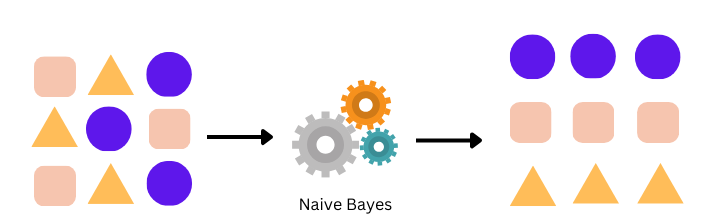
\includegraphics[width=1\textwidth]{img/Naive Bayes.png}
    \caption{Naive Bayes}
    \label{fig:Naive Bayes}
\end{figure}
\begin{figure}[H]
    \centering
    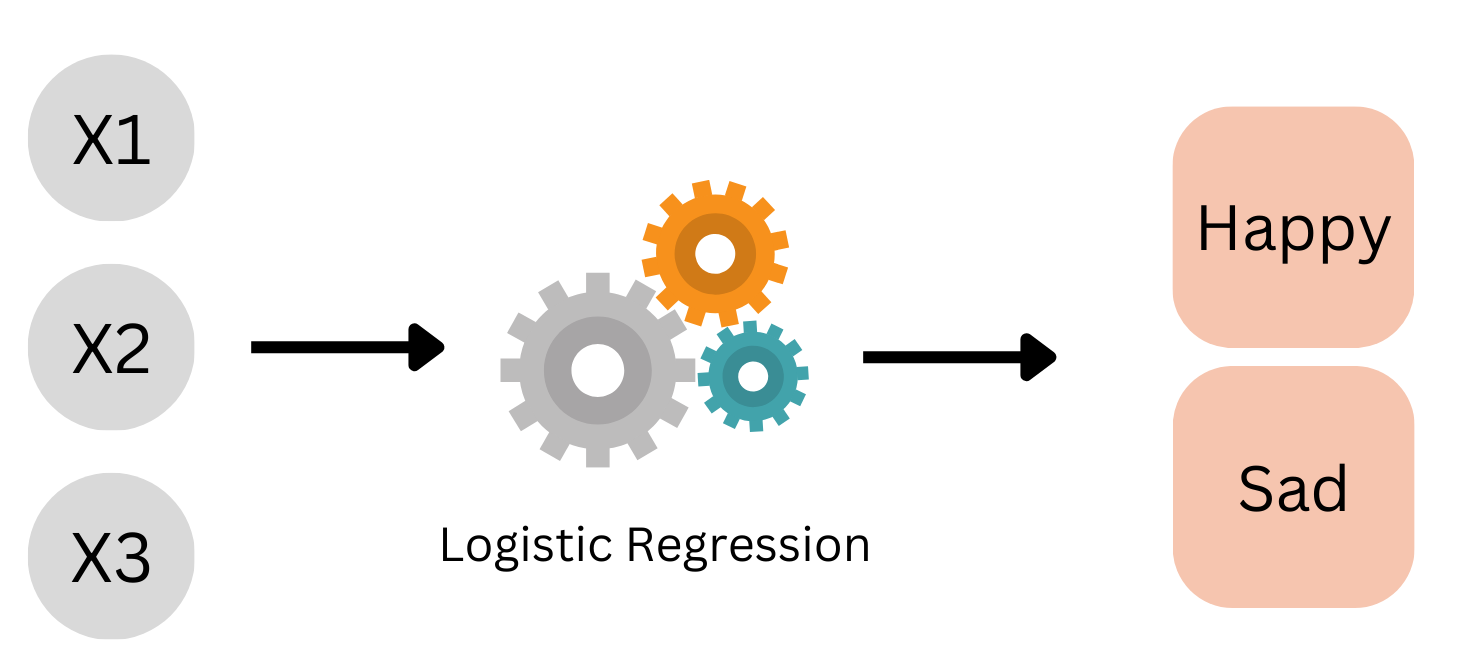
\includegraphics[width=.8\textwidth]{img/Logistic Regression.png}
    \caption{Logistic Regression}
    \label{fig:Logistic Regression}
\end{figure}
\subsubsection{Model Evaluation}

The models are assessed using metrics such as accuracy, precision, recall, F1-score, and AUC-ROC.
Feature importance analysis is conducted to identify the most significant predictors of churn.

\begin{figure}[H]
    \centering
    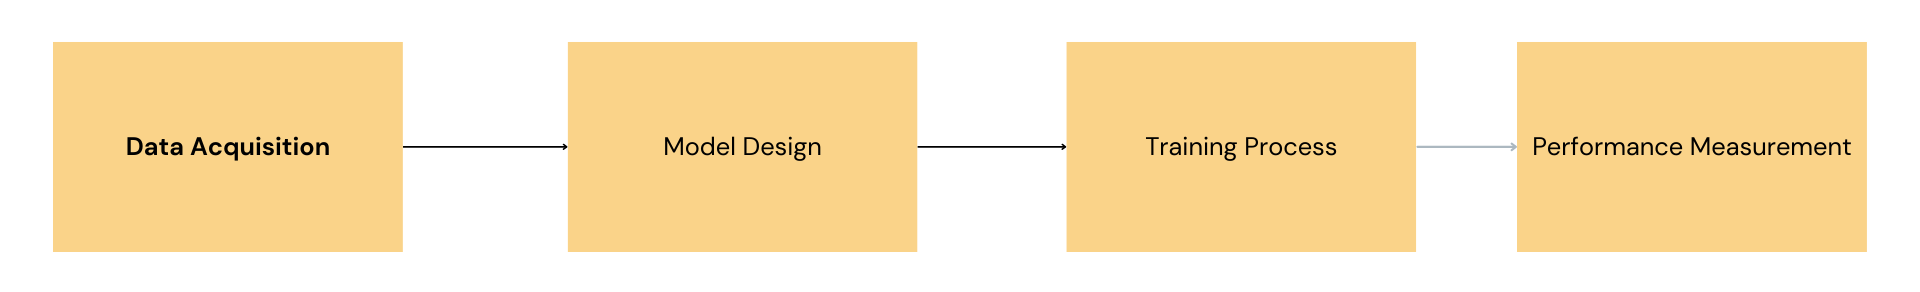
\includegraphics[width=1\textwidth]{img/model 1.png}
    \caption{Methodology of \cite{Agarwal2022-cq}}
    \label{fig:Methodology of paper 3}
\end{figure}

\subsection{Neural Network-based Individual and Ensemble Models}
\subsubsection{Data Collection and Preprocessing}

The dataset used is collected from a telecommunication company, including customer information and service usage data.
Preprocessing steps include handling missing values, normalization, and encoding categorical variables.
\subsubsection{Model Development}

Individual models: Various neural network architectures are explored, including Multi-Layer Perceptron (MLP).
Ensemble models: Combining multiple neural networks to form ensemble models using techniques such as bagging and boosting.
\begin{figure}[H]
    \centering
    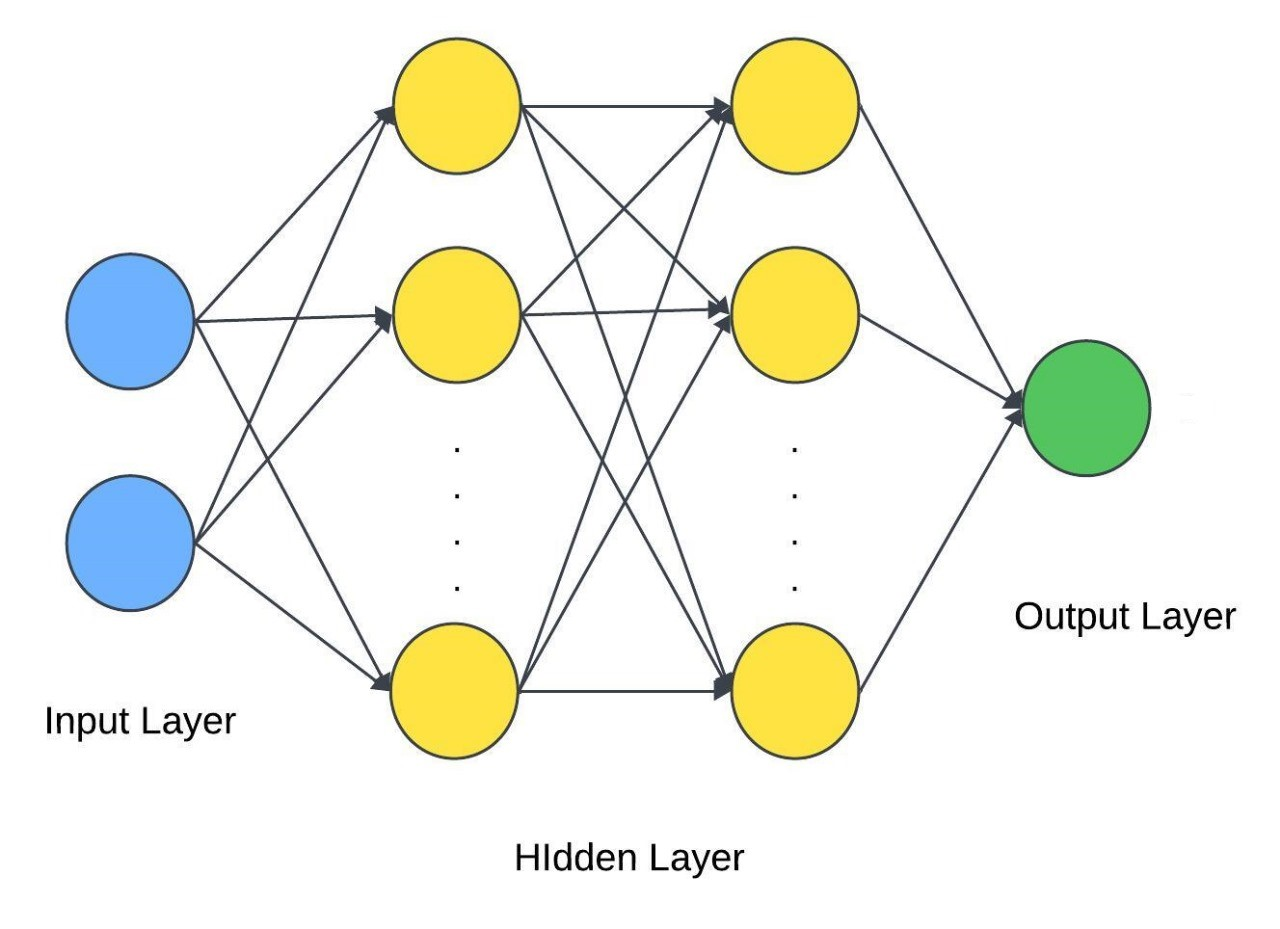
\includegraphics[width=.8\textwidth]{img/NN.jpg}
    \caption{Neural Network}
    \label{fig:Neural Network}
\end{figure}
\begin{figure}[H]
    \centering
    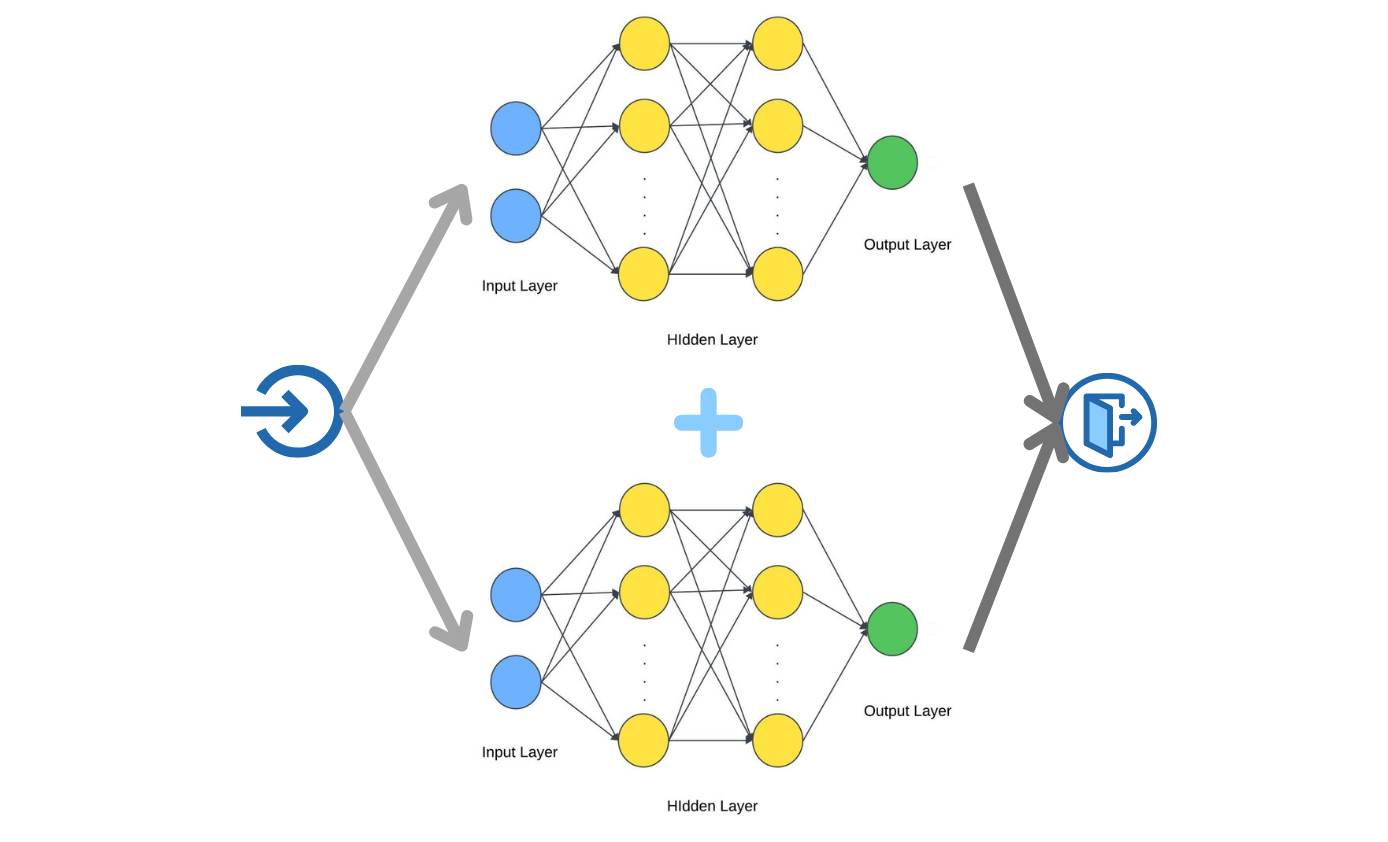
\includegraphics[width=1\textwidth]{img/ensemble.png}
    \caption{Ensemble of Neural Networks}
    \label{fig:Ensemble}
\end{figure}

\subsubsection{Training and Validation}

The dataset is split into training and validation sets.
Cross-validation is performed to fine-tune hyperparameters and prevent overfitting.
\subsubsection{Evaluation Metrics}

Models are evaluated using metrics such as accuracy, precision, recall, F1-score, and Area Under the Receiver Operating Characteristic Curve (AUC-ROC).\\\\

\begin{figure}[H]
    \centering
    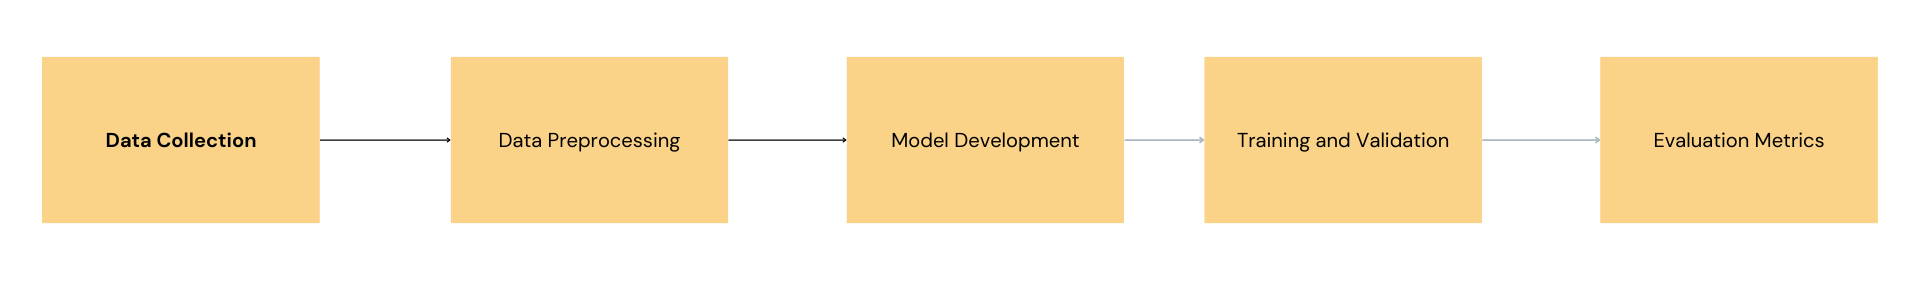
\includegraphics[width=1\textwidth]{img/model 2.png}
    \caption{Methodology of \cite{TSAI200912547}}
    \label{fig:Methodology of paper 2}
\end{figure}

\subsection{Hybrid Neural Networks}

\subsubsection{Data Acquisition}

Data is sourced from a telecom company, containing customer demographics, account information, and usage patterns.
Feature Engineering:

Relevant features are selected based on domain knowledge.
Data transformation techniques like normalization and categorical encoding are applied.
\subsubsection{Model Design}

Hybrid neural network models are designed by combining different types of neural networks, such as Convolutional Neural Networks (CNN) and Recurrent Neural Networks (RNN).
The hybrid model aims to capture both spatial and temporal patterns in the data.

\begin{figure}[H]
    \centering
    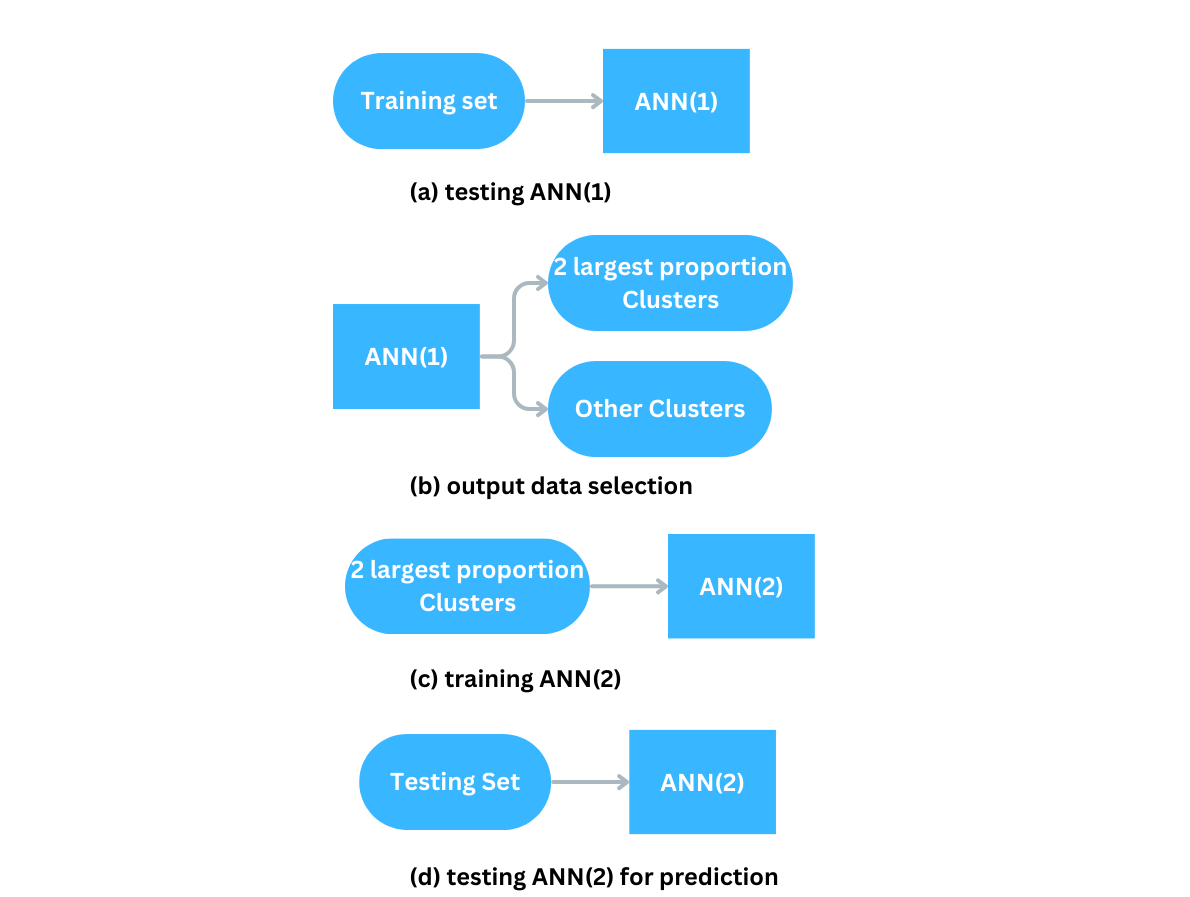
\includegraphics[width=.9\textwidth]{img/ANN+ANN.png}
    \caption{ANN+ANN Ensemble Model}
    \label{fig:ANN+ANN}
\end{figure}
\begin{figure}[H]
    \centering
    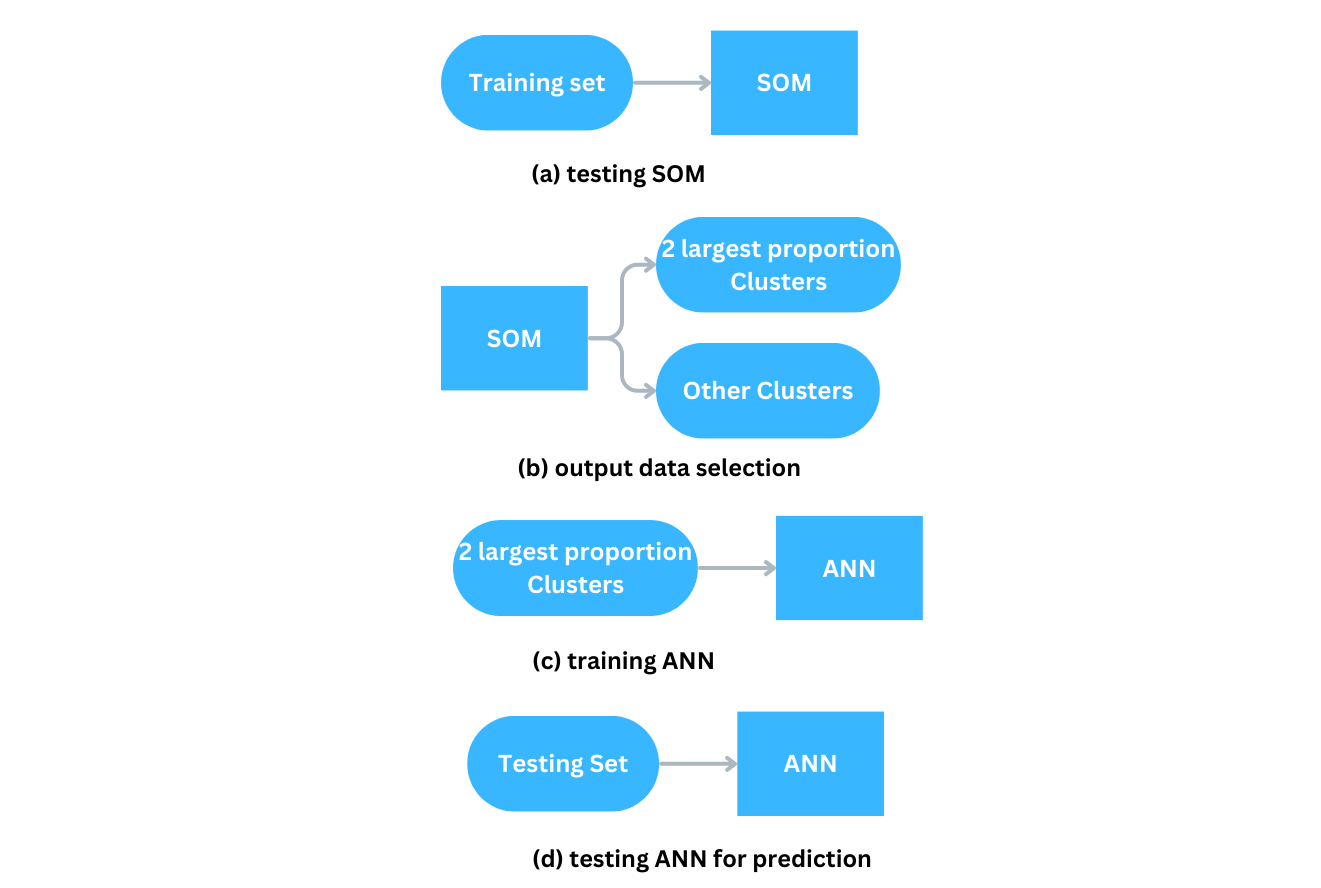
\includegraphics[width=.9\textwidth]{img/SOM+ANN.png}
    \caption{SOM+ANN Ensemble Model}
    \label{fig:SOM+ANN}
\end{figure}

\subsubsection{Training Process}

The dataset is divided into training, validation, and test sets.
Techniques like dropout and batch normalization are used to improve model generalization.
\subsubsection{Performance Measurement}

Evaluation is based on confusion matrix metrics: accuracy, precision, recall, F1-score, and AUC-ROC.
Comparative analysis is done with baseline models.\\\\

\begin{figure}[H]
    \centering
    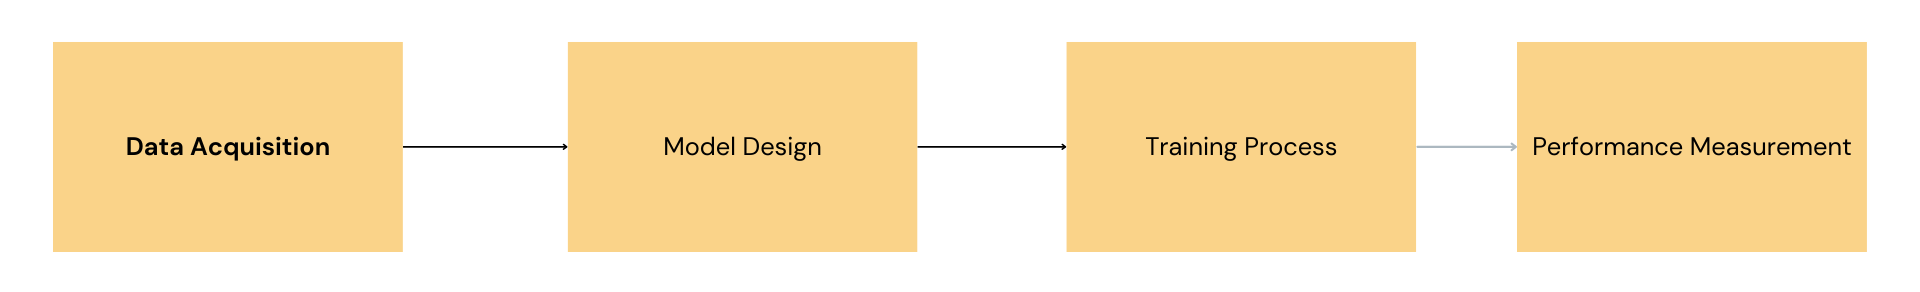
\includegraphics[width=1\textwidth]{img/model 1.png}
    \caption{Methodology of \cite{8667113}}
    \label{fig:Methodology of paper 1}
\end{figure}

